\chapter {Graph Theory}
\label{chap:graphTheory}
\myTop{This chapter concerns the graph theory in relation to the Rubik's Cube. 
The shortest path of a graph and the calculation of the diameter of a graph will be described.
This can be used as a method to prove how many twists are needed to solve the Rubik's Cube from any position, also called the upper bound.
The chapter will end with an example using a much smaller Rubik's Cube graph; the Middle movement graph.}

A graph consists of a set of vertices, $V$ \cite[p. 592]{Rosen07}, and a set of edges, $E$. There are several types of graphs, but in this chapter only simple graphs are described. 
A vertex is a point. A vertex can be connected to other vertices by an edge.
An edge is a line between two vertices(an edge can in some graphs connect a vertex to it self, called a loop, but such graphs are not taken into consideration here). Figure \ref{fig:generalDescriptionGraph} illustrates the basic principles of a graph.
\begin{figure}[ht]
	\centering
		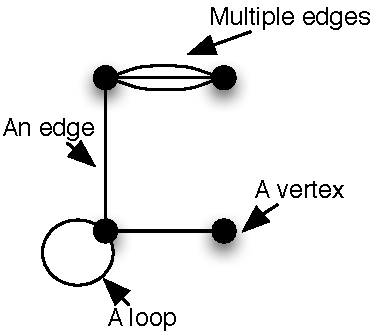
\includegraphics[scale = 0.7]{input/pics/generalDescriptionGraph.pdf}
	\caption{\myCaption{This is a graph with multiple lines and a loop. The graph is connected, but not simple.}}
	\label{fig:generalDescriptionGraph}
\end{figure}

If there is only one edge between any two vertices in a graph, then the graph is said to be simple.
A graph is said to be connected if you can visit every vertex by starting at an arbitrary vertex and then reach every other vertex by traveling along the edges of the graph. Figure \ref{fig:simpleUnconnectedGraph} illustrates an unconnected graph while figure \ref{fig:simpleConnectedGraph} illustrates a connected graph. 

Graphs can be directed. This means that the edges has a direction and travel can only be done along an edge in one direction. Figure \ref{fig:simpleDirectionalGraph} illustrates a directional graph. 

A graph can be weighted, which means that every edge will have a weight.
This weight can represent different things, distance between vertices, price for traveling between vertices or what ever makes sense for the given weighted graph.

\begin{figure}[htb]
	\centering
		\subfloat[\myCaption{A simple connected graph.}]{\label{fig:simpleConnectedGraph}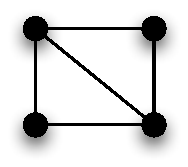
\includegraphics[width=0.15\textwidth]{input/pics/simpleConnectedGraph.pdf}}
		\hspace{0.2\textwidth}
		\subfloat[\myCaption{A simple unconnected graph.}]{\label{fig:simpleUnconnectedGraph}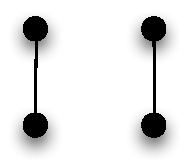
\includegraphics[width=0.15\textwidth]{input/pics/simpleUnconnectedGraph.pdf}}
		\hspace{0.2\textwidth}
		\subfloat[\myCaption{A simple directed graph}]{\label{fig:simpleDirectionalGraph}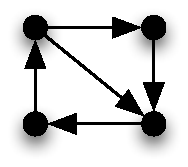
\includegraphics[width=0.15\textwidth]{input/pics/simpleDirectionalGraph.pdf}}
		\caption{\myCaption{Two simple graphs and one simple directed graph.}}
		\label{fig:cross}
\end{figure}

Graphs can be used to illustrate many different things such as different relationships, geographical maps, and tournaments.\cite[pp. 592-593]{Rosen07} 

For a graph of the \rubik{} it would be ideal to make vertices represent positions and edges represent \twist{}s. The weight of the edges would then be the number of \twist{}s required to get from one vertex of the edge to the other -- hence the weight for every edge would be 1 if only edges representing a single \twist{} is included in the graph.
%This means the graph is undirected, has no loops and there can only be one edge between two vertices. 
%Since all weights in the \rubik{} graph is $1$ the graph can be considered non-weighted.

The \rubik{} graph can have different sizes depending on the allowed \twist{}s, e.g. a graph only considering Rm2, Um2 and Fm2 \twist{}s can be made into a relatively small graph compared to the full \rubik{} graph(see \ref{fig:graphMiddleSlice2} for illustration), which contains $4.33 \cdot 10^{19}$ vertices.

%%Uddyb forklaring af rubik's cube som graf

\section{Shortest Path}
The shortest path from one vertex to another in a graph can be found by checking the length of each possible path. 
This is easy for a small graph such as the \nameref{sub:middleMoveGraph} \ref{sub:middleMoveGraph}, which will be described later in this chapter. For a bigger graph such as the full \rubik{} graph this is practically impossible. 
%%Mikael rettet her til
The shortest path between two vertices can be found by using e.g. Dijkstra's Algorithm \cite[p. 651]{Rosen07}. The description of the algorithm is omitted for brevity. Dijkstra's Algorithm takes an weighted graph and two vertices as input. 
Because of this the \rubik{} graph has to be weighted. Since each \twist{} contributes to the total number of \twist{}s by the same number, one, each edge is given the weight 1. The weight will be omitted in every illustration in this chapter because they are all 1.  

\section{Solving the Diameter}
To find the diameter of a graph is to find the longest shortest path between any two vertices in the given graph i.e. the shortest path with the highest value. 
This can be done by using Dijkstra's Algorithm on every set of vertices in the graph. 
This can be applied to the \rubik{} graph as well in order to find the maximum number of \twist{}s to solve the \rubik{} in the worst case scenario. %Unfortunately this approach is not viable because of the tremendous amount of positions the \rubik{} has even when considering symmetries.

%The diameter of the \rubik{} graph can be found be finding where the upper and lower bound meet with some other method.

\section{Describing the Cube as a Graph}
In order to describe the \rubik{} as a graph it is necessary to determine the edges and the vertices. For the \rubik{} graph edges are defined to represent \twist{}s and vertices to represent the positions. 
The full \rubik{} graph is indeed a simple graph. A move can be reversed which means that the graph is undirected. In order to get from a position $a$ to an adjacent position $b$ one can get there by a single move. 
The full \rubik{} graph consists of approximately $4.33\cdot10^{19}$ vertices -- all having $18$ edges.
It is practically impossible to draw this graph. Therefore the graph will be explained with a much simpler graph; the Middle Movement graph.


\subsection{The Middle Movement Graph}
\label{sub:middleMoveGraph}
This graph is a \rubik{} graph consisting of only the moves that \twist{} the middle sections. 
This is Rm2 Fm2 Um2. Note: Rm2 = R2 L2.  This graph is fairly small, since it only consists of eight vertices and 12 edges. See figure \ref{fig:graphMiddleSlice2}. \cite[pp. 158-167]{Rubik87}

\begin{figure}[bht!]
	\centering
		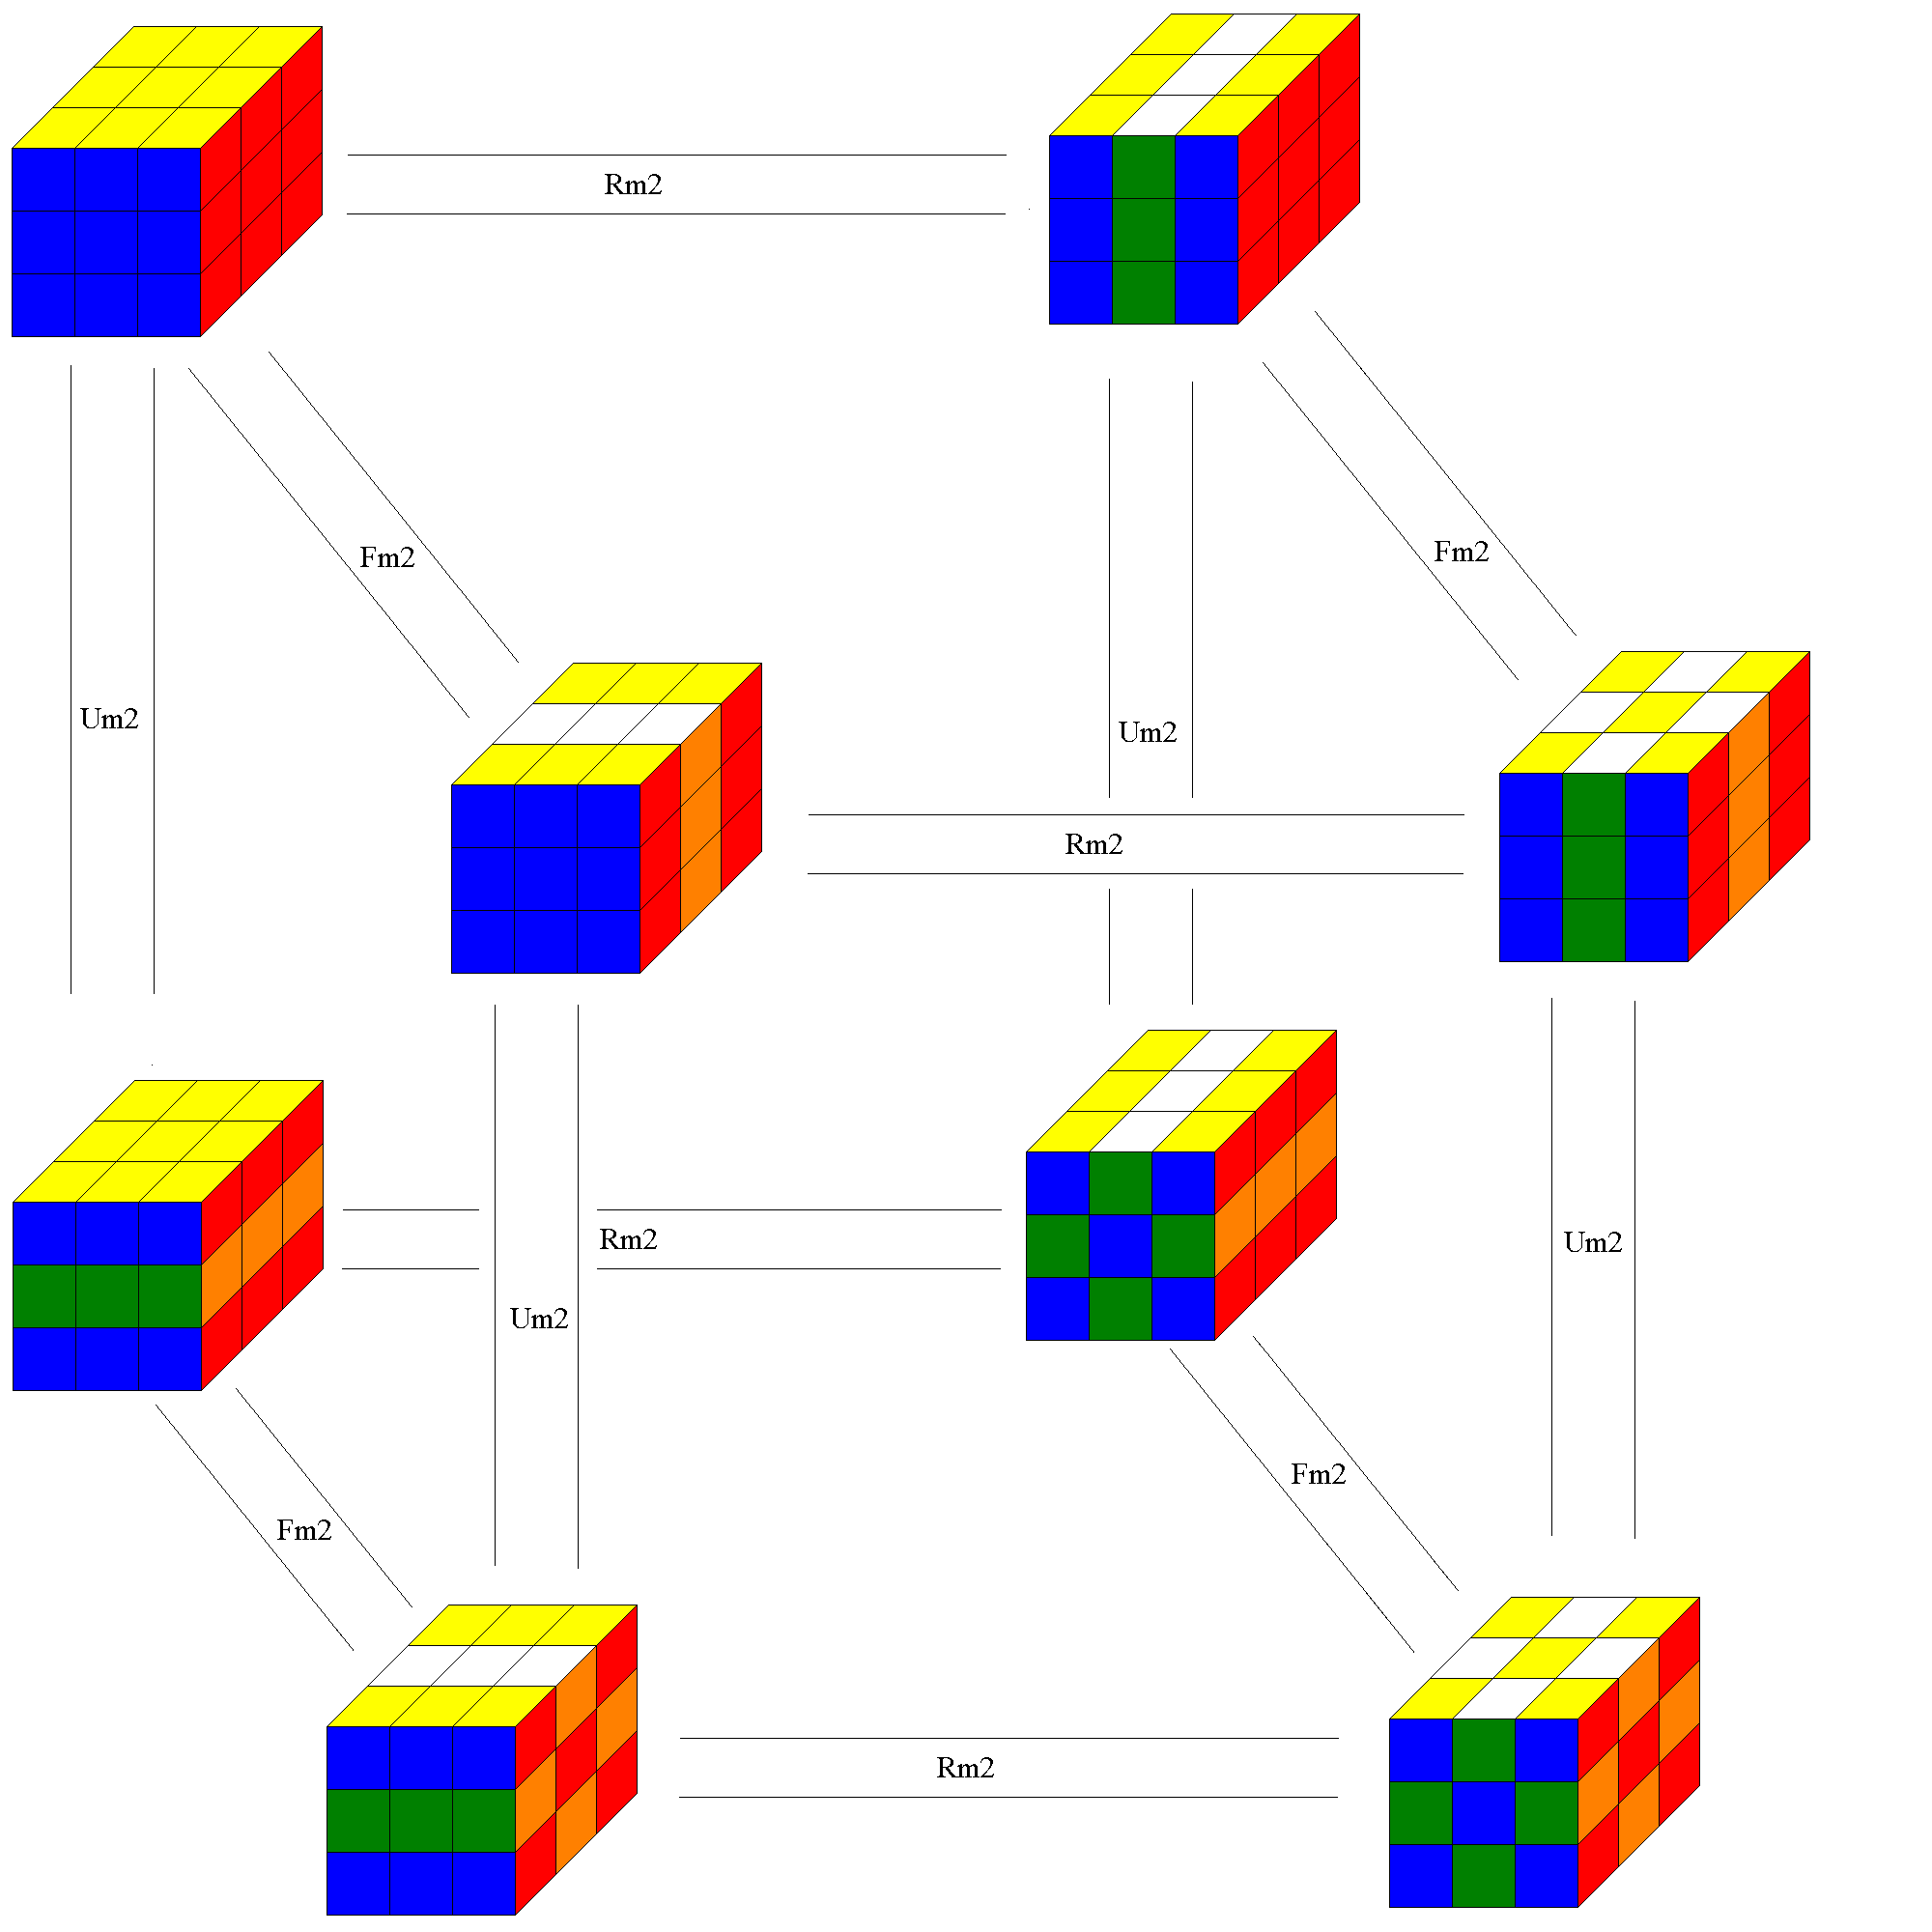
\includegraphics[width = 0.7\textwidth]{input/pics/graphMiddleSlice2.PNG}
	\caption{\myCaption{The graph of the middle movement positions.}}
	\label{fig:graphMiddleSlice2}
\end{figure}

Because of this graphs relatively small size the computation of the diameter is a somewhat simple task. It is possible to calculate the distance from all vertices to all other vertices, but since the graph is clearly symmetrical many calculations can be omitted. It is easy to see that the diameter must go from one corner to an opposite corner e.g. from the solved state to the pons asinorum\footnote{Pons asinorum is obtained from the solved state of a Rubik's Cube by the move sequence Rm2 Fm2 Um2.}. The diameter here is 3. 

In the full \rubik{} group it is believed that the analogous position to the pons asinorum, the superflip position, is the position which has the longest shortest path \cite{speedsolving.wiki}. This has however never been proven. This shortest path from the superflip to the solved position is 20\cite{rokicki09}.

\myTail{A short general description of graph theory has been presented in this chapter along with a way to calculate the diameter of a graph. For better understanding the theory, an example on applying the theory on the Rubik's Cube has been shown.}